\section{Theory}
In this section the theoretical background for this experiment is explained.
\textbf{Ein klein bisschen allgemeinen shit}
In cryptography the sender is refered to as Alice and the reciever is refered to as Bob. 
\textbf{One Time Pad}
\subsection{Polarisation states of photons}
\textbf{Malus und so}
\subsection{Quantum cryptography with the BB84 protocol}
For the BB84 protocol in quantum cryptography photon polarisation states can be used to transmitt information. 
For that two different bases (+ and x) are used. 
These two bases are at an angle of $\frac{\pi}{2}$ to each other. 
Then for each base one state is defined as the bit $0$ and the other orthogonal state is defined as the bit $1$ \cite{bennet_2014}. 
This encoding scheme is shown in \autoref{fig:encode_bb84}.
\begin{figure}
    \centering
    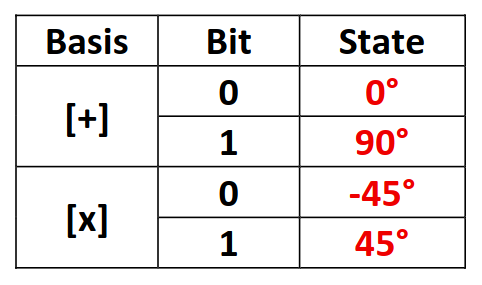
\includegraphics[width=0.4\textwidth]{images/encode_bb84.png}
    \caption{Encoding table for the BB84 protocol with photon polarisation states \cite{V29}.}
    \label{fig:encode_bb84}
\end{figure}
\FloatBarrier
To transmitt messages with this scheme, a key has to be generated first. 
In order to do so some bits have to be send. 
For each transmitted bit Alice and Bob will chose a base indiviually and randomly. 
Then Alice and Bob share their used bases publicly and toss away every bit, where their bases differ. 
The rest of these bits will be used as the key \cite{bennet_2014}.  %Quelle sollte passen 
\\
\textbf{Eve}



%\subsection{Uncertainties of the measurement}
%\label{sec:fehlerrechnung}
%%\subsection{Mittelwert}
%The mean value is calculated with
%\begin{equation}
%\bar{x} = \frac{1}{N} \sum_{i=1}^{N} x_i \, .
%\label{eqn:mittelwert}
%\end{equation}
%%\subsection{Standardabweichung}
%\\
%The standard deviation is given by
%\begin{equation}
%\sigma = \sqrt{\frac{1}{N - 1} \sum_{i=1}^{N} \left( x_i - \bar{x}_N \right)^2} \, .
%\label{eqn:standardabweichung}
%\end{equation}
%%%\subsubsection{Standardabweichung des Mittelwerts}
%The standard deviation of the mean value is given by
%\begin{equation}
%\Delta \bar{x} = \frac{\sigma}{\sqrt{N}} \, .
%\label{eqn:standardmittelwert}
%\end{equation}
%%%\subsection{Gaußsche Fehlerfortpflanzung}
%The deviation of a value derived from experimental parameters can be calculated using the Gaussian error propagation
%\begin{equation*}
%\Delta f = \sqrt{\sum_{i=1}^{N} \left( \frac{\partial f}{\partial x_i} \right)^2 \cdot (\Delta x_i)^2} \, .
%\label{eqn:fehlerfortpflanzung}
%\end{equation*}
%The relative deviation of an experimental parameter from the theoretical parameter is given by~\cite{relabw}
%\begin{equation}
%    \increment x_{\mathrm{rel}} = \left| \frac{x_{\mathrm{\exp}}-x_{\mathrm{theo}}}{x_{\mathrm{theo}}}\right|\, .
%    \label{eqn:relabw}
%\end{equation}

